\documentclass[onecolumn]{article} % article 文档类型

\usepackage[UTF8]{ctex}  % 使用宏包(为了能够显示汉字)

%代码块宏包
\usepackage{listings}
\usepackage{xcolor}

\definecolor{codegreen}{rgb}{0,0.6,0}
\definecolor{codegray}{rgb}{0.5,0.5,0.5}
\definecolor{codepurple}{rgb}{0.58,0,0.82}
\definecolor{backcolour}{rgb}{0.95,0.95,0.92}

\lstdefinestyle{mystyle}{
    backgroundcolor=\color{backcolour},   
    commentstyle=\color{codegreen},
    keywordstyle=\color{magenta},
    numberstyle=\tiny\color{codegray},
    stringstyle=\color{codepurple},
    basicstyle=\ttfamily\footnotesize,
    breakatwhitespace=false,         
    breaklines=true,                 
    captionpos=b,                    
    keepspaces=true,                 
    numbers=left,                    
    numbersep=5pt,                  
    showspaces=false,                
    showstringspaces=false,
    showtabs=false,                  
    tabsize=2
}

\lstset{style=mystyle}


%设置文章标题
\title{密码学作业1}  % 文章标题
\author{赵伯俣2021302181156}   % 作者的名称
\date{\today}       % 当天日期

\usepackage[a4paper,left=10mm,right=10mm,top=15mm,bottom=15mm]{geometry}

%插入图片的宏包
\usepackage{graphicx}
\usepackage{subcaption}


\begin{document}
%%----------- 主体部分 ----------- %%

\maketitle
\section{vigenere密码的加密程序}
以下将介绍使用vigenere密码的加密程序将一段明文加密成相应的密文

\subsection{编写思路}
    首先将明文中的空格去掉,只保留明文中的字母,然后利用vigenere的方法将明文的下标与密文的下标相加之后模除26即可得到密文的下标,
    将密文输出即可。

\subsection{源代码}
    \lstinputlisting[language=Python, caption=vigenere加密程序代码]{codes/vigenere1.py}

\newpage
\subsection{结果演示}
    \subsubsection{加密过程1}
        明文为:I am alive here, my beloved, for the reason to adore you. Oh!How anxious I have been 
        for you and how sorry I am about all you must have suffered in having no news from us. May 
        heaven grant that this letter reaches you. Do not write to me, this would compromise all of 
        us and above all,do not return under any circumstances. It is known that it was you who helped 
        us to get away from here and all would be lost if you should show yourself.We are guarded day 
        and night. I do not care you are not here. Do not be troubled on my account. Nothing will happen
        to me. The national assemble will show leniency. Farewell the most loved of men. Be quiet if you
        can take care of yourself.For myself I cannot write any more, but nothing in the world could 
        stop me to adore you up to the death.\\
        密钥为:hongye\\
        得到的密文如下图所示
        \begin{figure}[htbp] %代表图片的插入位置h:当前位置,t页面顶部,b页面底部,p浮动页
            \centering    %图片居中
            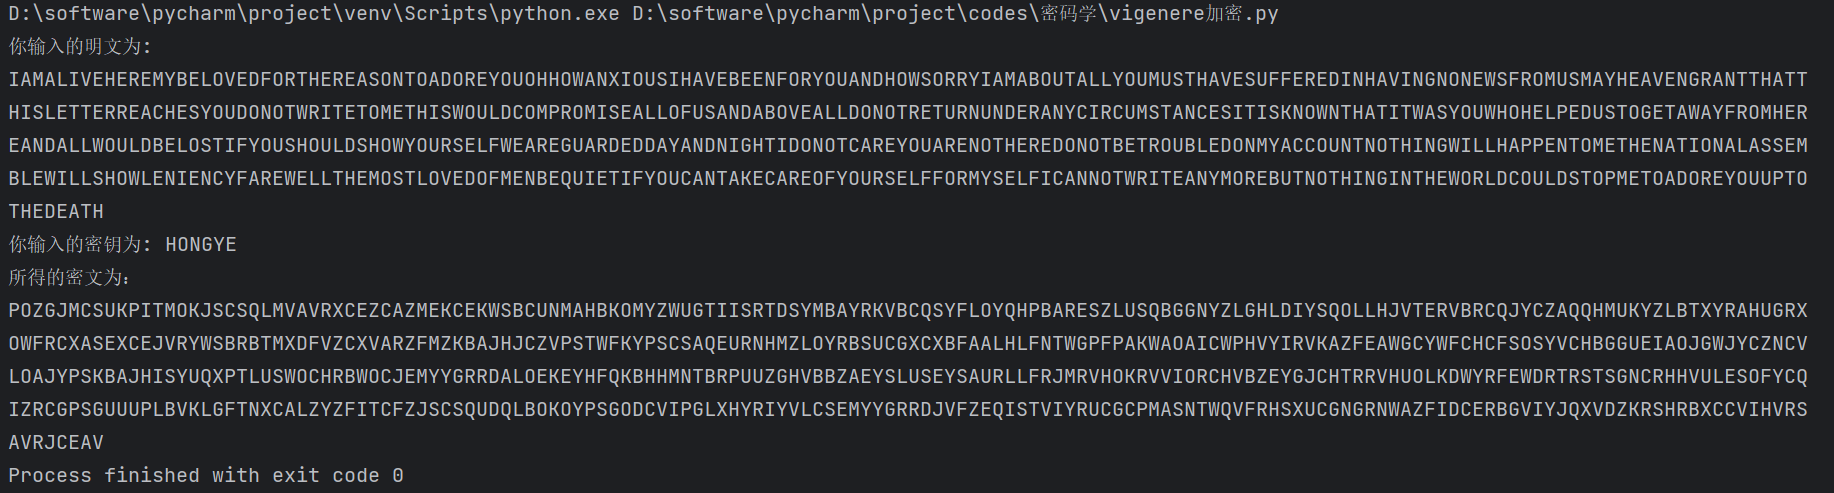
\includegraphics[width=18cm]{images/vigenere_result_1.png}  %[可选参数设置图片的宽高]
            \caption{加密程序运行结果1}    %图片标题
            \label{pic1}        %图片标签
        \end{figure}

    \subsubsection{加密过程2}
        明文为:It was the best of times.It was the worst of times. It was the age of wisdom. It was the 
        age offoolishness. It was the epoch of belief. It was the epoch of incredulity. It was the season
        of light. It was the season of darkness. It was the spring of hope. It was the winter of despair.
        We had everything before us. We had nothing before us. We were all going direct to heaven. We were 
        all going direct the other way. In short, the period was so, far like the present period, that some 
        of its noisiest authorities insisted on its being received, for good or for evil, in the superlative 
        degree of comparison only.\\
        密钥为:hongye\\
        得到的密文如下图所示
        \begin{figure}[htbp] %代表图片的插入位置h:当前位置,t页面顶部,b页面底部,p浮动页
            \centering    %图片居中
            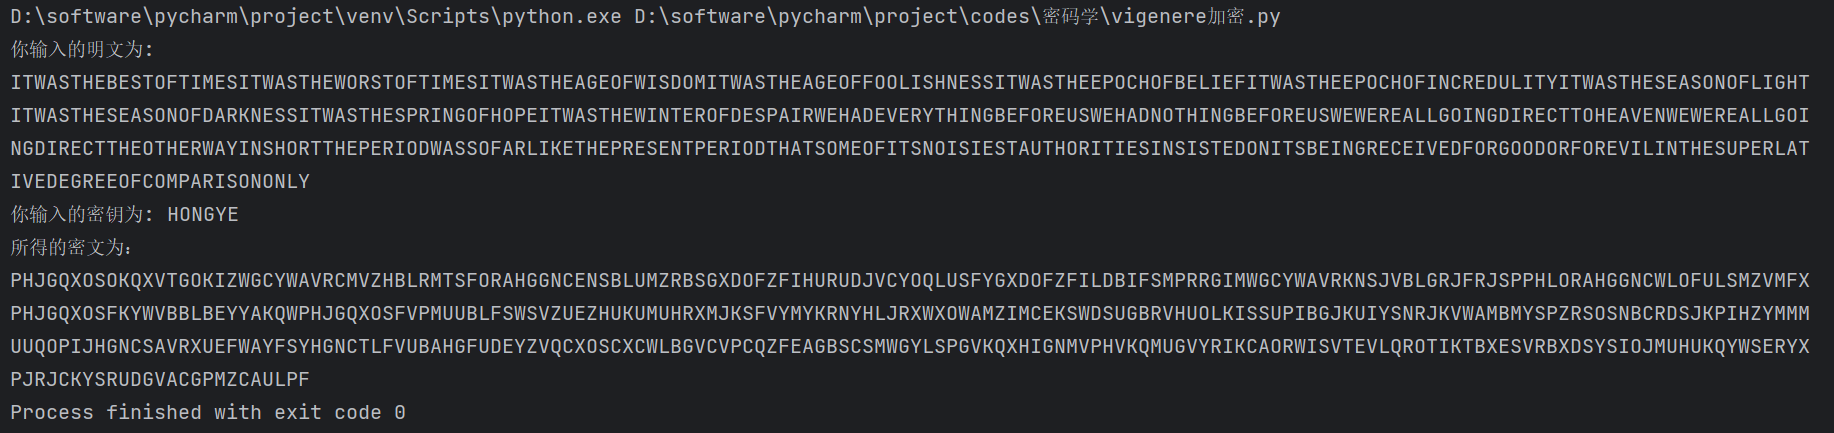
\includegraphics[width=18cm]{images/vigenere_result_2.png}  %[可选参数设置图片的宽高]
            \caption{加密程序运行结果2}    %图片标题
            \label{pic1}        %图片标签
        \end{figure}
    

\section{vigenere密码破译程序}
    以下将介绍在已知vigenere密码的密文的情况下破解其明文以及密钥

\subsection{编写思路}
    \subsubsection{通过重合指数法破解密钥的长度}
        在将密文中的空格去除之后通过find\_key\_len函数遍历从2到50的所有的密钥长度,假设当前遍历的密钥长度为i,
        则将密文分成i组,对于每一组调用count\_key\_len\_CI函数求其重合指数,得到密钥长度为i时的重合指数,因为每一个
        密钥长度对应有数组重合指数,所以在该次实验中调用Bias函数将当前密钥长度的重合指数求其对于0.065的偏差,
        取偏差最小的一组的密钥长度为该密文的密钥长度。\\   

    \subsubsection{通过互重合指数确定密钥字符之间的相对位移}
        在得到了密钥的长度key\_len之后通过调用group\_k函数将密钥字符串分成key\_len组,通过count\_MIC函数
        求得每一组与第一组之间的互重合指数表,并选取表中互重合指数最接近0.065的值的下标作为当前字符相对于第一个
        字符的偏移量,从而得到所有字符相对于第一个字符的偏移量。\\

    \subsubsection{遍历26种密钥字的情况选出合适的密钥字}
        该过程遍历26种密钥的情况,将密文的前二十位字符拿出用26种密钥分别进行解密,将解密的结果进行分词处理,由
        程序员选出最为符合语义的一个密钥并将其输入程序。\\

    \subsubsection{将密文字符串通过密钥转换为明文并做英文的分词处理}
        该步骤是在已知密文已知密钥的情况下将密文字符串进行翻译从而得到明文字符串,然后将得到的明文字符串进行
        分词处理,从而得到一个通顺的句子。\\
\newpage

\subsection{源代码}
    \lstinputlisting[language=Python, caption=vigenere破解程序代码]{codes/vigenere2.py}

\newpage
\subsection{代码运行结果演示}
    \subsubsection{破译过程1}
        已知密文为:\\

        \begin{lstlisting}
        cbkznkiyjsrofgnqadnzuqigscvxizgsjwucusrdkxuahgzrhywtvdjeiuwsrrtnpszbvpzncngztbvsrnzuqigscvf
        jwqgjwcytwdazuqigscvfjwqgjwjhkfdylmcbmhonbmbvdnvbmwbnacjaphhonbmbvdnvbmwbnaublsbdnjjneoroyf
        mxfhixpzpcozzuqigscvxcvhdmfgxmgovzsqmvzyvwyzmsczoajsejifoakdcrehwhgdehvmtnmvvmesvzifutzfjzo
        alwqztunwvdvmfhesvzifutzfjzoalwqztunpsnoyfleoxdetbwfsoyfjmfhjuxuagnarsfqydoyfjzsrzeujmfhjuu
        bihrjdfinwsnepcawdnkbobvnmzucmghijjmbscjejnapddehlmqddmfxncqbfpxwfejifpqzhikiyaiozimubwuzuf
        azsdjwdiudzmztivcmgp
        \end{lstlisting}

        破译结果如下图所示\\
        求得密钥长度和偏移量后遍历26种可能的密钥结果
        \begin{figure}[htbp]
            \centering 
            \begin{subfigure}[b]{0.4\textwidth}
                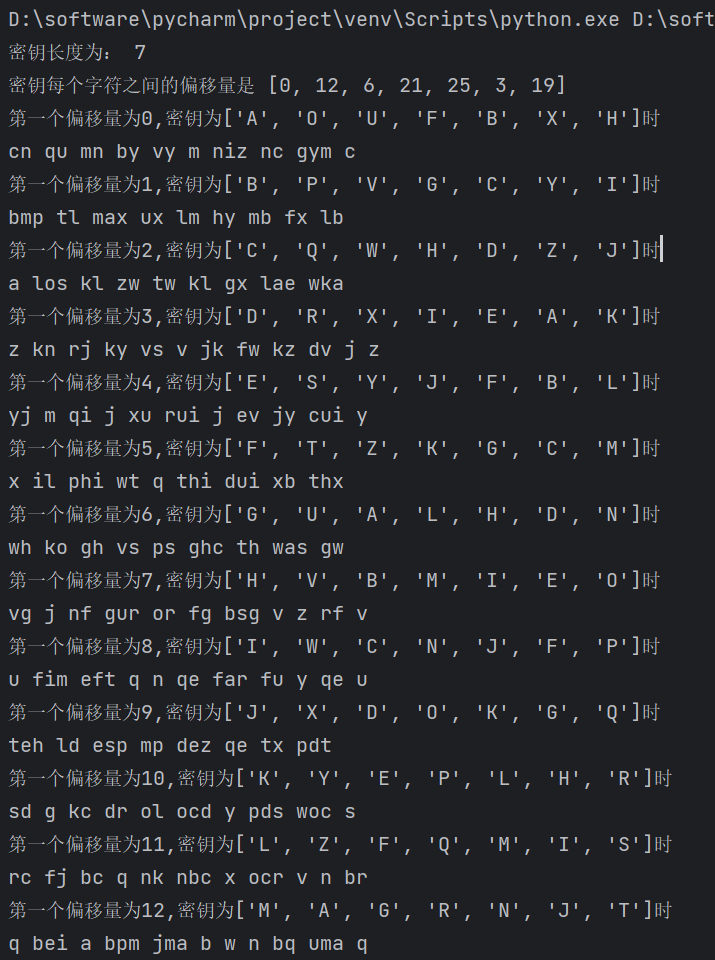
\includegraphics[width=\textwidth]{images/vigenere2_result_1.1.png}
                \label{fig:subfig1}
            \end{subfigure}
            \hfill
            \begin{subfigure}[b]{0.5\textwidth}
                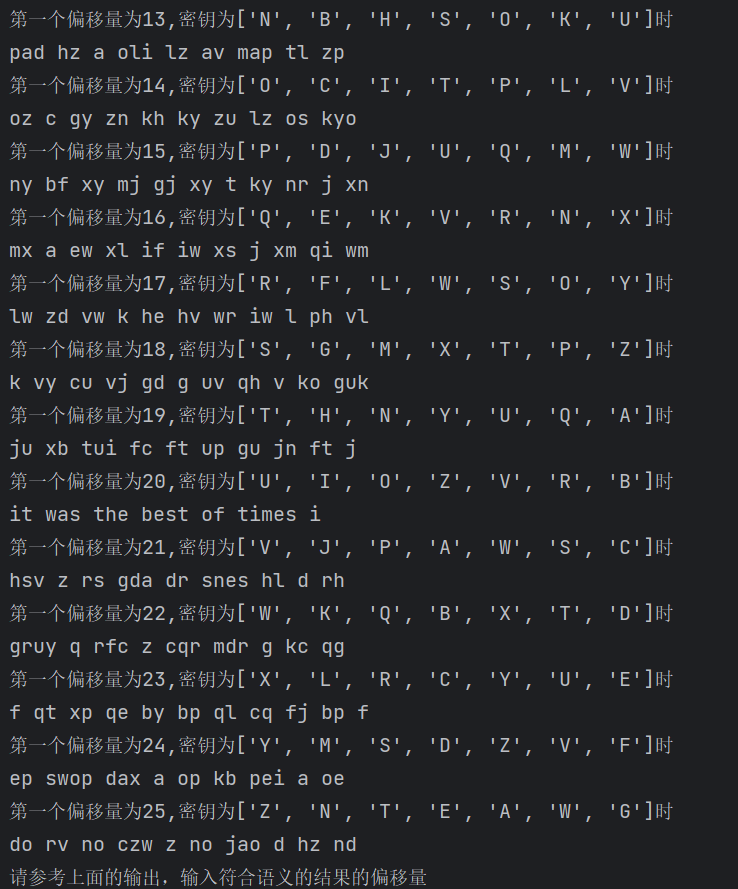
\includegraphics[width=\textwidth]{images/vigenere2_result_1.2.png}
                \label{fig:subfig2}
            \end{subfigure}
        
            \caption{密钥长度,偏移量和26种密钥运行结果}
            \label{fig:subfigures}
        \end{figure}

        选择最为符合语义的密钥结果后输出相应的明文如下图所示
        \begin{figure}[htbp] %代表图片的插入位置h:当前位置,t页面顶部,b页面底部,p浮动页
            \centering    %图片居中
            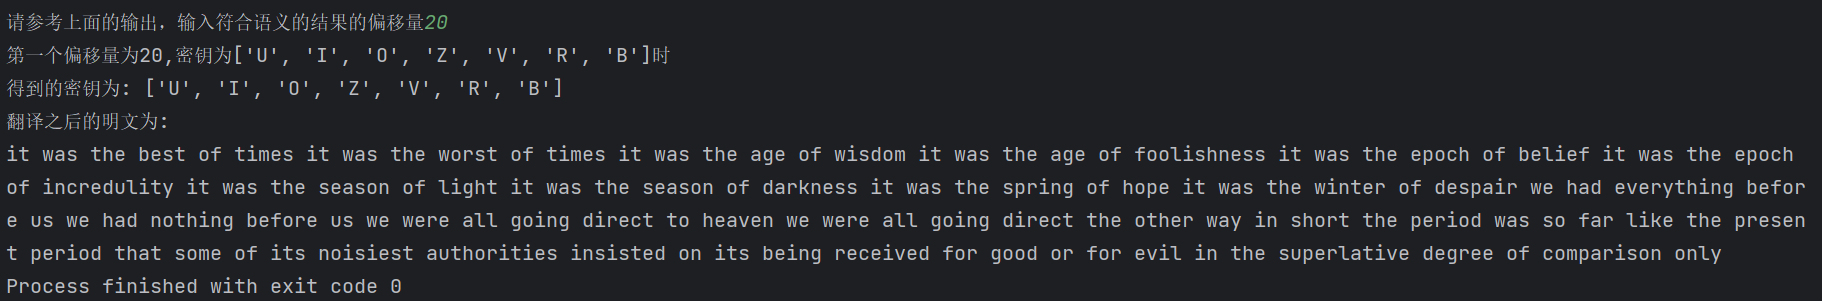
\includegraphics[width=18cm]{images/vigenere2_result1.3.png}  %[可选参数设置图片的宽高]
            \caption{得到明文结果}    %图片标题
            \label{pic1}        %图片标签
        \end{figure}
    \newpage
    \subsubsection{破译过程2}
        已知密文为:\\
        \begin{lstlisting}
            krkpekmcwxtvknugcmkxfwmgmjvpttuflihcumgxafsdajfupgzzmjlkyykxdvccyqiwdncebwhyjmgkazybtdf
            sitncwdnolqiacmchnhwcgxfzlwtxzlvgqecllhimbnudynagrttgiiycmvyyimjzqaxvkcgkgrawxupmjwqemi
            ptzrtmqdciakjudnnuadfrimbbuvyaeqwshtpuyqhxvyaeffldmtvrjkpllsxtrlnvkiajfukycvgjgibubldpp
            kfpmkkuplafslaqycaigushmqxcityrwukqdftkgrlstncudnnuzteqjrxyafshaqljsljfunhwiqtehncpkgxs
            pkfvbstarlsgkxfibffldmerptrqlygxpfrwxtvbdgqkztmtfsqegumcfararhwerchvygczyzjaacgntgvfktm
            jvlpmkflpecjqtfdcclbncqwhycccbgeanyciclxncrwxofqieqmcshhdccughsxxvzdnhwtycmcbcrttvmurql
            phxnwddkopqtehzapgpfrlkkkcpgadmgxdlrchvygczkerwxyfpawefsawukmefgkmpwqicnhwlnihvycsxckf
        \end{lstlisting}

        破译结果如下图所示
        求得密钥长度和偏移量后遍历26种可能的密钥结果
        \begin{figure}[htbp]
            \centering 
            \begin{subfigure}[b]{0.4\textwidth}
                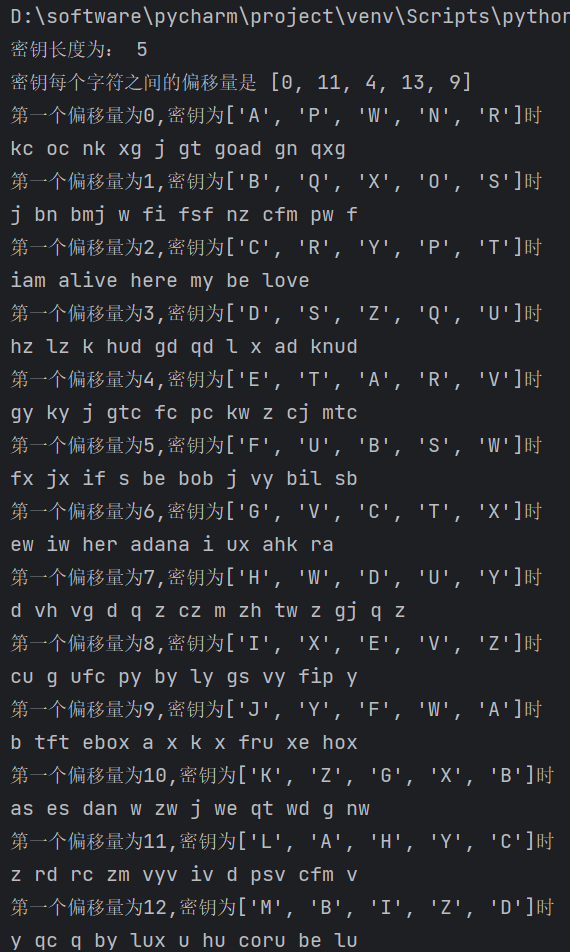
\includegraphics[width=\textwidth]{images/vigenere2_result2_1.1.png}
                \label{fig:subfig1}
            \end{subfigure}
            \hfill
            \begin{subfigure}[b]{0.4\textwidth}
                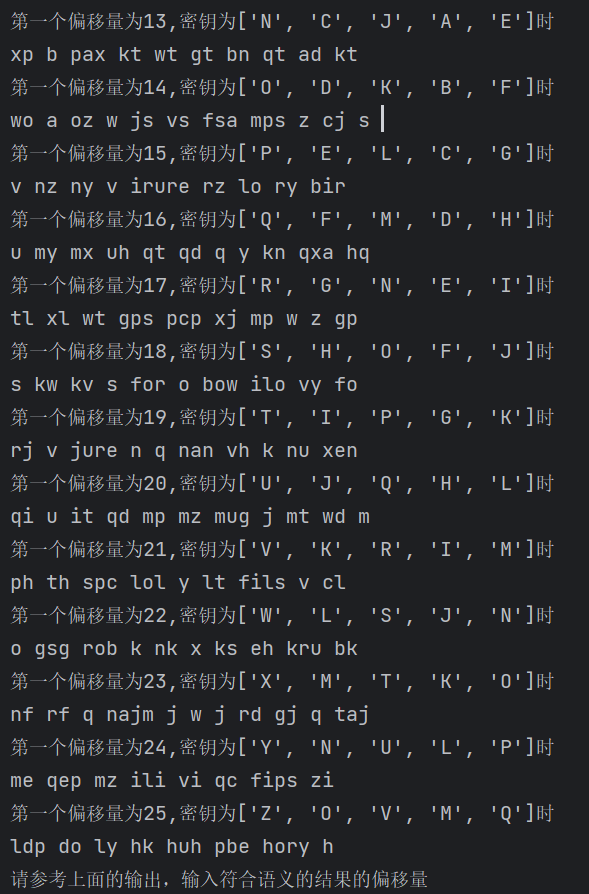
\includegraphics[width=\textwidth]{images/vigenere2_result2_1.2.png}
                \label{fig:subfig2}
            \end{subfigure}
        
            \caption{密钥长度,偏移量和26种密钥运行结果}
            \label{fig:subfigures}
        \end{figure}

        选择最为符合语义的密钥结果后输出相应的明文如下图所示
        \begin{figure}[htbp] %代表图片的插入位置h:当前位置,t页面顶部,b页面底部,p浮动页
            \centering    %图片居中
            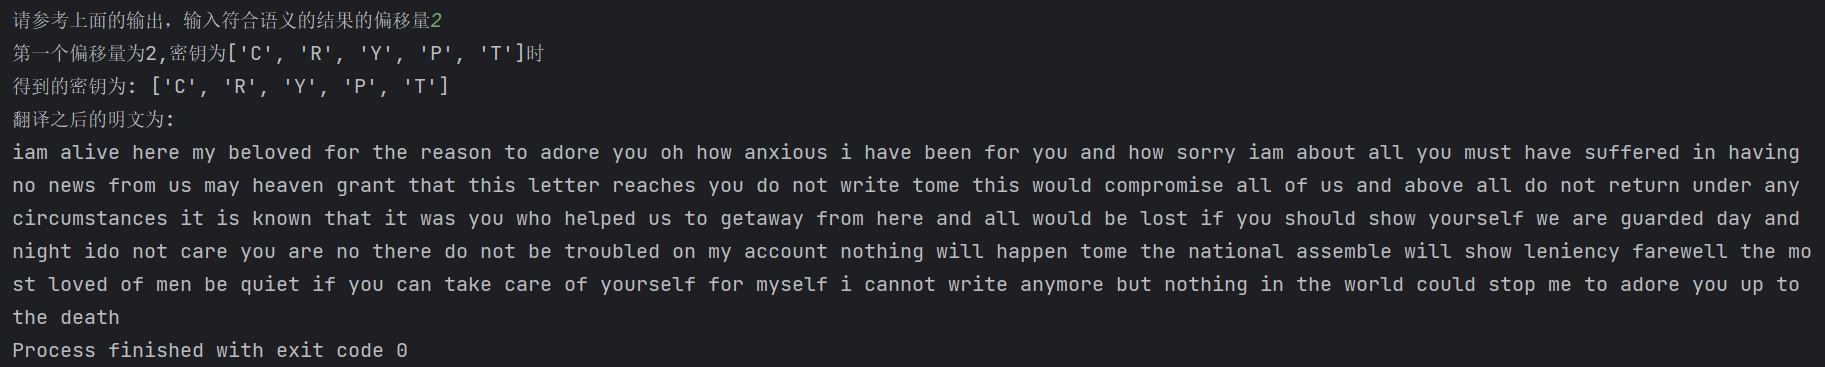
\includegraphics[width=18cm]{images/vigenere2_result2_1.3.png}  %[可选参数设置图片的宽高]
            \caption{得到明文结果}    %图片标题
            \label{pic1}        %图片标签
        \end{figure}

% Chapter 3

\chapter{引用与链接}

\section{脚注}
注释是对论文中特定名词或新名词的注解。注释可用页末注或篇末注的一种。选择页末注的应在注释与正文之间加细线分隔,线宽度为 1 点,线的长度不应超过纸张的三分之一宽度。同一页类列出多个注释的,应根据注释的先后顺序编排序号。字体为宋体5号,注释序号以“\circled{1}、\circled{2}”等数字形式标示在被注释词条的右上角。页末或篇末注释条目的序号应按照“\circled{1}、\circled{2}”等数字形式与被注释词条保持一致,脚注序号每面更新。示例:这里有个注释\footnote{我是解释注释的}。

\section{引用文中小节}\label{sec:ref}
如引用小节~\ref{sec:ref}

\section{引用参考文献}
这是一个参考文献引用的范例:“\cite{江泽民1989能源发展趋势及主要节能措施}提出……”。还可以引用多个文献:“\cite{kuhn2004man,江泽民2008新时期我国信息技术产业的发展,江泽民1989能源发展趋势及主要节能措施}提出……”。不同的引用方法:“\citet{江泽民1989能源发展趋势及主要节能措施}”“\citep{江泽民2008新时期我国信息技术产业的发展}”更多引用命令请参阅 natbib 文档或 biblatex 文档。\nocite{*}

文献引用需要配合 BibTeX 使用,很多工具可以直接生成 BibTeX 文件(如 EndNote、NoteExpress、百度学术、谷歌学术等),此处不作介绍。

\section{链接相关}
模板使用了 hyperref 包处理相关链接,使用 \verb|\href| 可以生成超链接,默认不显示链接颜色。如果需要输出网址,可以使用 \verb|\url| 命令,示例:\url{https://github.com}。

\end{document}
